\documentclass[12pt]{article}
%\usepackage[utf8]{inputenc}
\usepackage[latin1]{inputenc}
\usepackage[spanish]{babel}
\usepackage{anysize}
\usepackage{graphicx}
\usepackage{amsmath}
\marginsize{1cm}{2cm}{2cm}{2cm}  
\title{Tema 3. Ecuaciones Diferenciales Ordinarias (1a. Parte)}
\author{M. en C. Gustavo Contreras May\'{e}n}
\begin{document}
\maketitle
A partir del problema 4, deber\'{a}s de graficar los datos que te devuelva el algoritmo num\'{e}rico.
\begin{enumerate}
\item Resuelve los siguientes problemas en $0 \leq t \leq 5$ mediante el m\'{e}todo de Euler hacia adelante y $h=0.01$. Eval\'{u}a los errores por comparaci\'{o}n con los valores exactos.\\
\begin{enumerate}
	\item $y'+ty=1$ \hspace{1.5cm} $y(0)=1$
	\item $y'+3y = e^{-t} \hspace{1.5cm} y(0)=1$
	\item $y'= (t^{2} - y)$\hspace{1.5cm} $y(0)=0.5$
	\item $y'+y \vert y \vert = 0 \hspace{1.5cm} y(0)=1$
	\item $y' + \vert y \vert^{1/2} = \sin(t) \hspace{1.5cm} y(0)=1$
\end{enumerate}
\item Un dep\'{o}sito c\'{o}nico contiene agua hasta $0.5$ m de altura a partir del fondo. el dep\'{o}sito tiene un orificio en el fondo, de $0.02$ m de radio. El radio del dep\'{o}sito est\'{a} dado por $r=0.25y$, donde $r$ es el radio y $y$ la altura medida desde el fondo. La velocidad del agua que pasa por el orificio est\'{a} dada por $v^{2}=2gy$. Por medio del m\'{e}todo de Euler hacia adelante ($h=0.001$), calcula cu\'{a}ntos minutos se tardar\'{a} en vaciar el dep\'{o}sito.
\item Un tubo en forma de U y $0.05$ m de radio se llena con agua, pero con una divisi\'{o}n de forma que el nivel del agua en la parte vertical de la izquierda es $0.2$ cm m\'{a}s alto que el de la parte vertical derecha. En el instante $t=0$ se retira la divisi\'{o}n. El nivel del agua de la parte izquierda $y_{a}A$, medido desde el plano intermedio entre las dos superficies, satisface la ecuaci\'{o}n
\[ Ly_{a}^{''} = -2 gy_{a} \]
donde $L$ es la longitud total del agua en el tubo, que mide $1$ m. Si se desprecia la fricci\'{o}n del tubo, calcula el nivel del agua por medio del m\'{e}todo de Euler haciaa adelante para $0 < t < 10$ s y determina cu\'{a}ndo alcanza $y_{a}$ su m\'{a}ximo y su m\'{i}nimo. Utiliza $h=0.001$.
\item Repite el problema anterior, pero ahora suponiendo que hay fricci\'{o}n en el tubo de forma que la ecuaci\'{o}n de movimiento es 
\[ Ly_{a}^{''} = -2 gy_{a} - \beta y_{a}{'}\]
donde $\beta=0.8$ m/s. Usa nuevamente $h=0.001$.
\item La densidad num\'{e}rica (n\'{u}mero de \'{a}tomos por cm$^{3}$) del yodo-135 (radiois\'{o}topo) satisface la ecuaci\'{o}n
\[ \frac{d}{dt} N_{i}(t) = - \lambda_{i} N_{i}(t)  \]
 donde $N_{i}$ es la densidad num\'{e}rica del yodo-135 y $\lambda_{i}$ es su constante de decaimiento, igual a $0.1044$ horas$^{-1}$. Si $N_{1}(0) = 10^{5}$ \'{a}tomos/cm$^{3}$ en el instante $t=0$, calcula $N_{i}$ en $t=1$ hora mediante el m\'{e}to de Euler hacia adelante. Usa $h=0.05$ de hora.
 \item El producto de decaimiento del yodo-135 es el xen\'{o}n-135, tambi\'{e}n es radioactivo. Su constante de decaimiento es $\lambda = 0.0753$ horas$^{-1}$. La densidad num\'{e}rica del xen\'{o}n satisface la ecuaci\'{o}n
\[ \frac{d}{dt} N_{x}(t) = - \lambda_{x}N_{x}(t) + \lambda_{i} N_{i}(t) \]
donde $N_{x}$ es la densidad num\'{e}rica del xen\'{o}n y $N_{i}$ es la densidad num\'{e}rica del yodo, definida en el problema anterior. Supongamos que $N_{x}(0) = 0$. Calcula $N_{i}$ y $N_{x}$, con base al m\'{e}todo modificado de Euler. (Puesto que las ecuaciones diferenciales son lineales, utiliza las soluciones que m\'{a}s se aproximen a cada intervalo de tiempo). Genera una lista con los valores para cada 2 horas hasta alcanzar las 50 horas. Usa $h=0.1$ hora.
\item
	\begin{enumerate}
		\item Un tanque de 50 galones de agua contiene sal con una concentraci\'{o}n de 10 onzas/gal\'{o}n. Con el fin de diluir el contenido de sal, se suministra agua pura a raz\'{o}n de 2 galones/minuto. Si el dep\'{o}sito tiene una mezcla uniforme y la misma cantidad de agua que entra sale del dep\'{o}sito cada minuto, la concentraci\'{o}n de sal satisface\\
\[ y'_{1}(t)= -\frac{2}{50}y_{1}, \hspace{1.5cm} y_{1}(0)=10 \]\\
donde $y_{1}(t)$ es la concentraci\'{o}n de sal en onzas/gal\'{o}n y $t$ es el tiempo en minutos. Usando el m\'{e}todo de Runge-Kutta de segundo orden y $h=1$ minuto para determinar cu\'{a}nto tiempo debe de transcurrir para que la concentraci\'{o}n de sal sea $1/10$ de su valor inicial.
		\item El agua que sale del tanque entra a otro tanque de 20 galones, en el cual tambi\'{e}n se vierte agua pura a raz\'{o}n de 3 galones/minuto y se mezcla bien. La concentraci\'{o}n de sal en el segundo tanque satisface
		\[ y'_{2}(t) = - \frac{3}{20} y_{2}(t) + \frac{2}{20} y_{1}(t), \hspace{1cm} y_{2}(0)=0 \]
		donde $y_{1}(t)$ es la concentraci\'{o}n de sal del tanque de 50 galones del problema anterior. Usa RK2 para determinar cu\'{a}ndo alcanza su m\'{a}ximo la concentraci\'{o}n de sal en el tanque de 20 galones. Supongamos que el segundo tanque tiene agua pura en instante $t=0$.
	\end{enumerate}
\item Se dispara un proyectil al aire con un \'{a}ngulo de $45^{\circ}$ con respecto al suelo, con $u=v=150 m/s$, donde $u$ y $v$ son las velocidades horizontal y vertical, respectivamente. Las ecuaciones de movimiento est\'{a}n dadas por
\begin{eqnarray*}
	u^{'} & = & -c Vu, \hspace{1.5cm} u(0)=150 m/s \\
	v^{'} & = & -g - cVv, \hspace{1.5cm} v(0)=150 m/s
\end{eqnarray*}
donde $u$ y $v$ son funciones del tiempo, $u=u(t)$ $y v=v(t)$ y
\begin{eqnarray*}
	V & = & \sqrt{u^{2} + v^{2}} \\
	c & = & 0.005 \hspace{2cm} \mbox{(coeficiente de arrastre)} \\
	g & = & 9.9 m/s^{2}
\end{eqnarray*}
Las ecuaciones de movimiento se pueden resolver mediante alguno de los m\'{e}todos de Runge-Kutta. La trayectoria del proyectil se puede determinar al integrar
\[ x' = u \hspace{2cm} \mbox{y} \hspace{2cm} y' = v \]
o bien
\begin{eqnarray*}
	x & = & \int^{t}_{0} u(t^{'}) dt^{'} \\
	y & = & \int^{t}_{0} v(t^{'}) dt^{'}
\end{eqnarray*}
Escribe un programa en Python con el m\'{e}todo RK2 que resuelva y grafique la trayectoria del proyectil.
\item Re-escribe el programa del problema anterior, pero ahora con el m\'{e}todo RK3.
\item El movimiento del sistema de masas que se muestra en la figura (1) est\'{a} dado por:
\[ y'' + 2 \zeta \omega y' + \omega^{2}y = \frac{F(t)}{M}\]
donde \\ 
$\omega = \left( \frac{k}{M} \right)^{2}$ (frecuencia natural sin amortiguamiento, $s^{-1}$) \\
$\zeta = \frac{c}{2M\omega}=0.5$ (factor de amortiguamiento) \\
$k = 3.2$ (constante del resorte, $\frac{kg}{s^{2}}$ \\
$M=5$ (masa, kg) \\
$F(t) = 0$ (fuerza, Newtons)
\begin{figure}[!h]
	\centering
	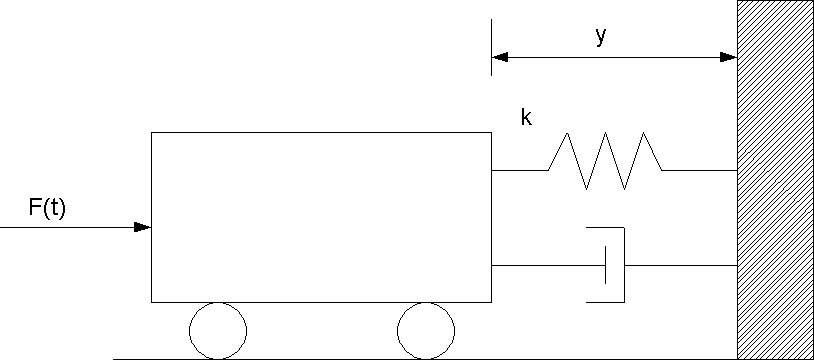
\includegraphics[scale=0.4]{Figura01.png}  
	\label{fig:figura01}
	\caption{Sistema masa-resorte.}
\end{figure}
\\Si $F(t)$ es una funci\'{o}n escalonada de magnitud $F_{0}=1$ kg y cuya duraci\'{o}n es 1 segundo, determina el movimiento de la masa para $0<t<10$ segundos por medio del m\'{e}todo de RK4.
\item Determina la respuesta y carga din\'{a}mica del sistema amortiguado del problema anterior sujeto a un pulso de fuerza triangular
\begin{equation*}
	F(t) =
		\begin{cases}
			2F_{0}t,  & 0 \leq t \leq 1 s\\
			2F_{0}(1-t), & 1 \leq t \leq 2 s\\
			0, & t>2 s
		\end{cases}
\end{equation*}
Donde $F_{0}=1$ Kg (fuerza). Utiliza el m\'{e}todo RK4.
\end{enumerate}
\end{document}
